\documentclass[12pt, oneside]{article}

\usepackage[letterpaper, scale=0.8, centering]{geometry}
\usepackage{fancyhdr}
\setlength{\parindent}{0em}
\setlength{\parskip}{1em}

\pagestyle{fancy}
\fancyhf{}
\renewcommand{\headrulewidth}{0pt}
\rfoot{{\footnotesize Copyright Daniel Grier / Mia Minnes, 2023, Version \today~(\thepage)}}

\usepackage{titlesec}

\author{CSE105Sp23}

\newcommand{\instructions}{{\bf For all HW assignments:} Weekly homework 
may be done individually or in groups of up to 3 students. 
You may switch HW partners for different HW assignments. 
The lowest HW score will not be included in your overall HW average. 
Please ensure your name(s) and PID(s) are clearly visible on the first page of your homework submission 
and then upload the PDF to Gradescope. If working in a group, submit only one submission per group: 
one partner uploads the submission through their Gradescope account and then adds the other group member(s) 
to the Gradescope submission by selecting their name(s) in the ``Add Group Members" dialog box. 
You will need to re-add your group member(s) every time you resubmit a new version of your assignment.
 Each homework question will be graded either for correctness (including clear and precise explanations and 
 justifications of all answers) or fair effort completeness. You may only collaborate on HW with CSE 105 students 
 in your group; if your group has questions about a HW problem, you may ask in drop-in help hours or post a private 
 post (visible only to the Instructors) on Piazza.

All submitted homework for this class must be typed. 
You can use a word processing editor if you like (Microsoft Word, Open Office, Notepad, Vim, Google Docs, etc.) 
but you might find it useful to take this opportunity to learn LaTeX. 
LaTeX is a markup language used widely in computer science and mathematics. 
The homework assignments are typed using LaTeX and you can use the source files 
as templates for typesetting your solutions.
To generate state diagrams of machines, we recommend using Flap.js
or JFLAP. Photographs of clearly hand-drawn diagrams may also be used. We recommend that you
submit early drafts to Gradescope so that in case of any technical difficulties, at least some of your
work is present. You may update your submission as many times as you'd like up to the deadline.


{\bf Integrity reminders}
\begin{itemize}
\item Problems should be solved together, not divided up between the partners. The homework is
designed to give you practice with the main concepts and techniques of the course, 
while getting to know and learn from your classmates.
\item You may not collaborate on homework with anyone other than your group members.
You may ask questions about the homework in office hours (of the instructor, TAs, and/or tutors) and 
on Piazza (as private notes viewable only to the Instructors).  
You \emph{cannot} use any online resources about the course content other than the class material 
from this quarter -- this is primarily to ensure that we all use consistent notation and
definitions (aligned with the textbook) and also to protect the learning experience you will have when
the `aha' moments of solving the problem authentically happen.
\item Do not share written solutions or partial solutions for homework with 
other students in the class who are not in your group. Doing so would dilute their learning 
experience and detract from their success in the class.
\end{itemize}

}

\newcommand{\gradeCorrect}{({\it Graded for correctness}) }
\newcommand{\gradeCorrectFirst}{\gradeCorrect\footnote{This means your solution 
will be evaluated not only on the correctness of your answers, but on your ability
to present your ideas clearly and logically. You should explain how you 
arrived at your conclusions, using
mathematically sound reasoning. Whether you use formal proof techniques or 
write a more informal argument
for why something is true, your answers should always be well-supported. 
Your goal should be to convince the
reader that your results and methods are sound.} }
\newcommand{\gradeComplete}{({\it Graded for completeness}) }
\newcommand{\gradeCompleteFirst}{\gradeComplete\footnote{This means you will 
get full credit so long as your submission demonstrates honest effort to 
answer the question. You will not be penalized for incorrect answers. 
To demonstrate your honest effort in answering the question, we ask 
that you include your attempt to answer *each* part of the question. 
If you get stuck with your attempt, you can still demonstrate 
your effort by explaining where you got stuck and what 
you did to try to get unstuck.} }

\usepackage{tikz}
\usetikzlibrary{automata,positioning,arrows}

\usepackage{amssymb,amsmath,pifont,amsfonts,comment,enumerate,enumitem}
\usepackage{currfile,xstring,hyperref,tabularx,graphicx,wasysym}
\usepackage[labelformat=empty]{caption}
\usepackage{xcolor}
\usepackage{multicol,multirow,array,listings,tabularx,lastpage,textcomp,booktabs}

\lstnewenvironment{algorithm}[1][] {   
    \lstset{ mathescape=true,
        frame=tB,
        numbers=left, 
        numberstyle=\tiny,
        basicstyle=\rmfamily\scriptsize, 
        keywordstyle=\color{black}\bfseries,
        keywords={,procedure, div, for, to, input, output, return, datatype, function, in, if, else, foreach, while, begin, end, }
        numbers=left,
        xleftmargin=.04\textwidth,
        #1
    }
}
{}

\newcommand\abs[1]{\lvert~#1~\rvert}
\newcommand{\st}{\mid}

\newcommand{\cmark}{\ding{51}}
\newcommand{\xmark}{\ding{55}}
 
\newcommand{\SUBSTRING}{\textsc{Substring}}
\newcommand{\REP}{\textsc{Rep}} 
\title{HW3 : Nonregular Languages and Pushdown Automata}
\date{Due: April 25th at 5pm (no penalty late submission until 8am next morning), via Gradescope}

\begin{document}
\maketitle
\thispagestyle{fancy}

\textbf{In this assignment:}

You will practice distinguishing between regular and nonregular languages using both 
closure arguments and the pumping lemma.

\textit{Resources}: To review the topics you are working with for this assignment, 
see the class material from Week 2 through Week 4. We will post frequently asked questions 
and our answers to them in a pinned Piazza post.

\textit{Reading and extra practice problems}: Sipser Section 1.4, 2.2. Chapter 1 
exercises 1.29, 1.30. Chapter 1 problems 1.49, 1.50, 1.51.

\textit{Key Concepts:} Pumping lemma, pumping length, regular languages, nonregular languages, 
pushdown automata, stack.

\instructions

You will submit this assignment via Gradescope
(\href{https://www.gradescope.com}{https://www.gradescope.com}) 
in the assignment called ``hw3CSE105Sp23''.

\textbf{Requests from your TAs and tutors}
To help us with grading please 
\begin{itemize}
    \item Start each question on a new page.
    \item Label the start of each solution with {\bf Answer}.
\end{itemize}

\textbf{Assigned questions}

\begin{enumerate} 



\item \textbf{Regular or not?} (21 points):\\
Fix $\Sigma = \{0,1\}$ and $\Gamma = \{0,1,2\}$.
For each of the languages listed below, 
prove that it is either regular or nonregular. {\it Note:} You might find it useful to 
explore the definition of each set and 
consider alternate (simpler) ways of stating it.

For each language that is regular, a complete 
solution will include a 
precise definition of a DFA, NFA, or regular 
expression that recognizes or describes it, along 
with a brief justification
of your construction by explaining the role each 
state plays in the machine
or referring back to relevant definitions.

For each language that is nonregular, a complete
solution will use the pumping lemma to prove that it is nonregular, 
including appropriate
justification related to the specific language.

\begin{enumerate}
    \item\gradeCorrectFirst $L_1 = \{0^n x 1^n \mid n \ge 1, x \in \Sigma^*\}$, a language over $\Sigma$.
    \item\gradeCorrect $L_2 = \{0^n 1 x 0 1^n \mid n 
    \ge 1, x \in \Sigma^* \}$, a language over 
    $\Sigma$.
    \item\gradeCorrect 
    Recall that for $L \subseteq \Sigma^*$, we define
    \begin{align*}
    \REP(L) &:= \{ w \in \Gamma^* \mid \text{between every pair of successive $2$'s in $w$ is a string in $L$}\}\\
    &\phantom{:}=\{w \in \Gamma^* \mid \text{for all } v \in \Sigma^* \text{ if } 2v2 \in \SUBSTRING(\{w\})  \text{, then } v \in L\} 
    \end{align*}
    $L_3 = \REP( \{ 0^n 1^n \mid n \geq 1 \} )$, 
    a language over $\Gamma$.
\end{enumerate}




\item \textbf{Properties of nonregular languages} (21 points): \\
Prove or disprove each of the following statements. In other words, decide whether 
each statement is true or false and justify your decision. 
Let $\Sigma = \{0,1\}$ and let $\Gamma = \{0,1,2\}$.
\begin{enumerate}
    \item\gradeCorrect For all languages $L, K$ over
    $\Sigma$, if $L$ is nonregular and $K$ is finite, then $L - K$ is nonregular.
    Recall: $L - K = \{ w \in \Sigma^* \mid w \in L \text{ and } w \notin K\}$.
    \item\gradeCorrect Every infinite language over $\Sigma$ 
    where each string in the language has an equal number of $0$'s and 
    $1$'s is nonregular.
    \item\gradeCorrect Recall that for language $K$ over $\Gamma$,
    \[
    \SUBSTRING(K) := \{ w \in \Gamma^* \mid \text{there exist } a,b \in \Gamma^* \text{ such that } awb \in K\}.
    \]
    For every nonregular language $K$ over $\Gamma$, $\SUBSTRING(K)$ is nonregular.
\end{enumerate}

\item \textbf{Pumping dilemma} (8 points): \\
Your friend claims that the Pumping Lemma is useless for proving that an infinite language 
$K \subseteq \Sigma^*$ is not regular. Their logic goes like this

\begin{enumerate}[label=(Step~\arabic*), leftmargin=2cm]
\item[(Step 1)] Suppose that $K$ is regular. It can be recognized by a 
DFA $M = (Q, \Sigma, \delta, q_0, F)$.
\item[(Step 2)] For arbitrary DFA $M$, the pumping length $p$ is at least $|Q|$.
\item[(Step 3)] However, for every integer $n \ge |Q|$, there exists a machine 
$M' = (Q', \Sigma, \delta', q_0', F')$ such that $L(M') = L(M) = K$ and $|Q'| = n$.
\item[(Step 4)] Therefore, the Pumping Lemma cannot be used to pump any string 
of finite length since its pumping length might be arbitrarily large.
\end{enumerate}

Below, we will examine the steps above in detail. Justify your answer to each part.
\begin{enumerate}
    \item\gradeCompleteFirst (Step 1): Is this statement true? In other words, just because we're assuming that $K$ is regular a regular language, does it mean we can assume there is a DFA that recognizes it?

    \item\gradeComplete (Step 2): 
    In general, it's true that the smallest the pumping length of a language
    recognized by a DFA with states $Q$ can be is $|Q|$. Prove this by finding a specific infinite language $K$ and a DFA recognizing 
    where $K$ cannot have pumping length smaller than $|Q|$.

    \item\gradeComplete (Step 3): This step is correct;
    prove the stated version of this statement: For every integer $n \ge |Q|$, there 
    exists a machine $M' = (Q', \Sigma, \delta', q_0', F')$ such that $L(M') = L(M)$ and $|Q'| = n$.

    (\textit{Challenge; not graded}): 
    Define a \emph{cycle} to be a sequence of \emph{distinct} states $q_1, q_2, \ldots, q_m$ such that
	\[
	\delta(q_1, \sigma_1) = q_2, \hspace{1cm} \delta(q_2, \sigma_2) = q_3, \hspace{.5cm} \ldots, \hspace{.5cm}\delta(q_m, \sigma_m) = q_1, 
	\]
	where $\sigma_1, \sigma_2, \ldots, \sigma_m \in \Sigma$ are symbols in the alphabet. 
    An objection to the statement in (Step 3) is that the proof of the Pumping Lemma 
    depends on the length of the cycles in the DFA rather than the number of states. That is, 
    increasing the number of states in your DFA might not increase the pumping length because 
    the length of the smallest cycle stays the same. Nevertheless, a version of your friend's statement 
    is still true whenever you impose this additional cycle constraint:  for every integer $n \ge |Q|$, 
    there exists a machine $M' = (Q', \Sigma, \delta', q_0', F')$ such that $L(M') = L(M)$ and the length 
    of the smallest cycle in the $M'$ is at least $n$. \\

	Your task is to show that even this more general statement is true for the simple language $\Sigma^*$ 
    recognized by the DFA below:
	\begin{center}
    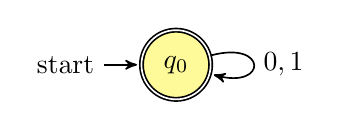
\begin{tikzpicture}[->,>=stealth',shorten >=1pt, auto, node distance=2cm, semithick]
    \tikzstyle{every state}=[text=black, fill=yellow!40]

    \node[initial,state, accepting] (q0) {$q_0$};

    \path (q0)  edge [loop right] node {$0,1$} (q0);
    \end{tikzpicture}
    \end{center}
	For all $n \ge 1$, define a DFA for this language where the length of the smallest cycle is $n$.

    \item\gradeComplete (Step 4): Describe why this statement is true/false/misleading.
\end{enumerate}


\end{enumerate}

\end{document}